\documentclass[a4paper,11pt]{article}
\usepackage{CAR}
\usepackage[T1]{fontenc}
\usepackage{amsfonts}
\usepackage{amsmath}
\usepackage{amssymb}
\usepackage{todo}

\begin{document}
\setcounter{footnote}{0}
\setcounter{figure}{0}


%%%%%%%%%%%%%%%%%%%%%%%%%%%%%%%%%%%%%%%%%%%%%%%%%%%%%%%%%%%%%%%%%%%%%%%%%%%%%%%%
% FOR THE AUTHORS
%%%%%%%%%%%%%%%%%%%%%%%%%%%%%%%%%%%%%%%%%%%%%%%%%%%%%%%%%%%%%%%%%%%%%%%%%%%%%%%%

\Aufsatz 
% Title
{Complexity of the Quantum Algebraic Attack on AES:\\
The Condition Number of the Macaulay Matrix}
% Short title for the table of contents
{Complexity of the Quantum Algebraic Attack on AES}
% Authors
{Dr. P. Nonnenmann, X. Bogomolec,}
% Label of authors' names
{NameAuthor}
% Names and adresses
{Dr. Peter Nonnenmann,
{\small \textit{DHBW Mannheim and Quant-X Security {\&} Coding}} \\
Dipl. Math. Xenia Bogomolec, 
{\small \textit{CEO Quant-X Security {\&} Coding}} \\}
% Images of authors
{./PQS_logo_pure_with.png}
% E-Mails
{peter.nonnenmann@quant-x-sec.com,xb@quant-x-sec.com,} 

\noindent
{\small \textit{With the friendly essential support of Prof. Dr. Siegfried Rump (Head of the Institute for Reliable Computing, TU Harburg) and Christoph Stockhammer (MathWorks)}}



%%%%%%%%%%%%%%%%%%%%%%%%%%%%%%%%%%%%%%%%%%%%%%%%%%%%%%%%%%%%%%%%%%%%%%%%%%%%%%%%
% IF THE ARTICLE IS WRITTEN IN ENGLISH, THEN UNCOMMENT
% THE NEXT LINE AND ANOTHER LINE AT THE END OF THIS FILE
\begin{otherlanguage}{english}
%%%%%%%%%%%%%%%%%%%%%%%%%%%%%%%%%%%%%%%%%%%%%%%%%%%%%%%%%%%%%%%%%%%%%%%%%%%%%%%%

\vspace{3mm}


%%%%%%%%%%%%%%%%%%%%%%%%%%%%%%%%%%%%%%%%%%%%%%%%%%%%%%%%%%%%%%%%%%%%%%%%%%%%%%%%
% WRITE YOUR ARTICLE BELOW using \Ueberschrift \Ueberschriftu \begin{figurehead}
%%%%%%%%%%%%%%%%%%%%%%%%%%%%%%%%%%%%%%%%%%%%%%%%%%%%%%%%%%%%%%%%%%%%%%%%%%%%%%%%

% The command \section{Title}{label} produces a headline and new section
\section{Abstract}

\noindent
\textit{We investigate the condition number of the Macaulay matrix in the Quantum Algebraic Attack \cite{QAA} on the symmetric cryptographic algorithm \textsc{AES} (Advanced Encryption Standard \cite{AES}). The Quantum Algebraic Attack is a quantum cryptanalysis, which can be applied to cryptographic algorithms based on polynomial systems that can be reduced to Boolean equation systems. \textsc{AES} is the standardized version of \textsc{Rijndael} and globally used for hybrid encryption in protocols such as TLS, OpenPGP, SSH, IPSec, etc. as well as for purely symmetric applications such as hard disk encryption. The S-Box of \textsc{Rijndael} is a polynomial system which can be reduced to a Boolean equantion system.} \\

\noindent
\textit{We show that the complexity of a Quantum Algebraic Attack on \textsc{AES} under the classical notion of a condition number $\kappa$ of a matrix equals infinity, independent of the key size. Therefore the application of Boolean equation solving \cite{QAA} on \textsc{AES} is not practical under these defined circumstances. } \\

\noindent
\textit{The computation of the modified notion of the condition number $\kappa$ of the involved Macaulay matrix requires the explicit generation of its derived reduced matrix and the computation of its condition number. These investigations are currently ongoing in our independent research project. } \\


\section{Introduction}

\noindent
It is known that currently used asymmetric cryptography relying on the hardness of integer factorization and discrete logarithm systems will no longer be valid with the advent of potent enough quantum computers. Quantum cryptanalyses on symmetric cryptography have been published far more recently, amongst them \\

\begin{itemize} [noitemsep, nolistsep]
  \item[1)] Quantum Algorithms for Boolean Equation Solving and Quantum Algebraic Attack on Cryptosystems \\
  \textbf{Chen-Gao quantum algorithm} \cite{QAA}.
  \vspace{0.1cm}
  \item[2)] A fast quantum mechanical algorithm for database search \\
  \textbf{Grover’s search algorithm} \cite{GRV}.
  \vspace{0.1cm}
\end{itemize}
\vspace{0.5cm}

\noindent
\textbf{Grover’s search algorithm} can be used to extract the key from a small number of \textsc{AES} plaintext-ciphertext pairs (e. g. $5$ for \textsc{AES}-$256$ \cite{GRO}). It is an alternative algorithm for an exhaustive key search (brute force attack). There are papers with quantum resource estimates for \textsc{AES} \cite{GRO}, \textsc{eAES} \cite{KUN, CEX}, \textsc{SHA-3} \cite{QSH} and \textsc{SHA-2} \cite{QSH}. \\

\noindent
The \textbf{Chen-Gao quantum algorithm} raised expectations to a harder impact on the security of \textsc{AES}. It is based on the \textsc{HHL} quantum algorithm \cite{HHL} and involves a quantum algebraic attack on cryptosystems, which can be reduced to Boolean equation solving. This attack reduces the security level of \textsc{AES}-$256$ from $256$ to $78.53$, with a factor \textit{c}, the complexity constant of the \textsc{HHL} algorithm and $\kappa^2$, the condition number of the Boolean equation system used in the algorithm. The condition number $\kappa$ depends on the cryptosystem which is solved by the Chen-Gao quantum algorithm. It has a quadratic impact on the complexity of \textsc{AES} because it stems from the S-Box, which is used twice within the algorithm: for the key schedule and during the block encryption/decryption. \\

\begin{figurehere}
  \centering
  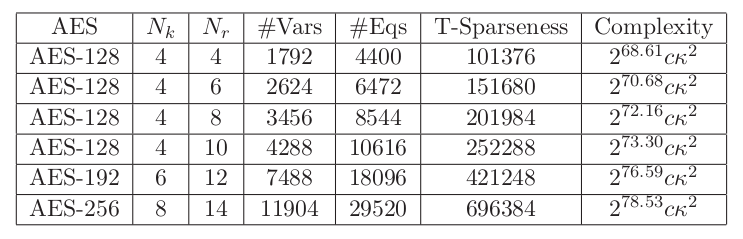
\includegraphics[width=12cm]{AES_table.png}
  \caption{Complexities of the Quantum Algebraic Attack on AES, table 2 \cite{QAA}.\label{abb_1}}
\end{figurehere}

\vspace{0.3cm} 
We investigate the condition number of \textsc{AES}-$256$. \\ 



\section{Chen-Gao Quantum Algorithm: A Quantum Algebraic Attack}

\noindent
The authors of \cite{QAA} present an algorithm which leads to new considerations of the security of systems which can be reduced to solving Boolean equations. A solution $a$ for the equation $\mathcal{F} \cdot a = 0$ with a set of polynomials $\mathcal{F} \subset \mathbb{C}[X], X = (x_1, \ldots, x_n) \,$ for an $ n \in \mathbb{N}$, is called \textit{Boolean} if each coordinate of $a$ is either $0$ or $1$. For the detailed description of the Chen-Gao quantum algorithm, we refer to the original paper \cite{QAA}.\\

\noindent
The resulting quantum algebraic attack algorithm includes quantum-monomial solving of polynomial systems over $\mathbb{C}$ by applying a Macaulay linear system. Like this they construct a Boolean equation solving algorithm, with the following properties: \\

\begin{itemize} [noitemsep, nolistsep]
  \item[1)] It decides if there exists a Boolean solution.
  \vspace{0.1cm}
  \item[2)] With a given probalility it finds a Boolean solution if there are such solutions to the system.
  \vspace{0.1cm}
  \item[3)] It returns $\emptyset$ if no Boolean solution exists.
\end{itemize}
\vspace{0.5cm}

\noindent
The matrix $A_{mca}$, which represents the Macaulay linear system of the attacked crypto system, defines the desired condition number $\kappa$. In order to derive $A_{mca}(AES)$ and then compute $\kappa$ of \textsc{AES}, we take a look at the structure of \textsc{AES}. The derived condition number $\kappa$ is that of the matrix $A_{mca}(AES)$.


\subsection{Structure of \textsc{AES}}

\noindent
\textsc{Rijndael} is a block cipher. That means that the basic encryption functions are iterated a certain number of rounds with dedicated round keys over the state. With $r = $ number of rounds, the encryption process is:\\

\begin{itemize} [noitemsep, nolistsep]
\item[(1)] \textbf{Derive round keys}\\
Call \textit{ExpandKey}\,(key) to derive $r+1$ round keys from the secret key. The $+ 1$ stands for the fact that \textit{Add\-RoundKey} is called additionally before each block encryption. 
\vspace{0.1cm}
\item[(2)] \textbf{Encryption}\\
Perform on each block of data represented by the \glqq state\grqq: 
\vspace{0.1cm}
  \begin{itemize} [noitemsep, nolistsep]
    \item[a)] Initial round:
      \begin{itemize} [noitemsep, nolistsep]
        \item[] Add the plaintext to the state 
        \item[] \textit{AddRoundKey}\,(state, $1$st round key)
      \end{itemize} 
    \vspace{0.1cm}
    \item[b)] For ($i=2$; $i\leq r-1$, $i$++):
    \vspace{0.1cm}
    \begin{itemize} [noitemsep, nolistsep]
        \item[] \textit{SubBytes}\,(state) 
        \item[] \textit{ShiftRows}\,(state) 
        \item[] \textit{MixColumns}\,(state) 
        \item[] \textit{AddRoundKey}\,(state, $i$-th round key) 
    \end{itemize} 
    \vspace{0.1cm}
    ($4$ basic \textsc{Rijndael} encryption functions)
    \vspace{0.1cm}
    \item[c)] The final round:
    \begin{itemize} [noitemsep, nolistsep]
        \item[] \textit{SubBytes}\,(state)
        \item[] \textit{ShiftRows}\,(state)
        \item[] \textit{AddRoundKey}\,(state, last round key) 
    \end{itemize} 
  \end{itemize}
\end{itemize}
\vspace{0.5cm}

The $4$ basic functions of the \textsc{Rijndael} encryption are: \\

\begin{itemize} [noitemsep, nolistsep]
  \item[1)] \textit{AddRoundKey} - addition in ${(\mathbb{F}_2)}^{128}$: \\ 
  Bitwise addition of the state and the correspondent round key.
  \vspace{0.1cm}

  \item[2)] \textit{SubBytes} - non-linear substitution: \\
  Each byte is replaced by another according to the specified substitution table ($S$-Box). A more resource friendly option is to treat a state byte as an element $\alpha \in \mathbb{F}_2 [x]/(x^8 + x^4 + x^3 + x + 1)$, where the multiplicative inverse of $\alpha$ needs to be found.
  \vspace{0.1cm}

  \item[3)] \textit{ShiftRows} - transposition for diffusion: \\
  The second, third and fourth row of the state are shifted to the left, by $1$, $2$ and $3$ steps.
  \vspace{0.1cm}

  \item[4)] \textit{MixColumns} - mixing for diffusion: \\
  Multiplication of each column of the state with the following matrix $M_{mix}$:

  $$ 
  	M_{mix} = 
  	\begin{bmatrix}
  		2 & 3 & 1 & 1 \\ 
  	 	1 & 2 & 3 & 1 \\
  	 	1 & 1 & 2 & 3 \\
  	 	3 & 1 & 1 & 2 \\
  	\end{bmatrix}
  $$

\end{itemize} 

\vspace{0.3cm}
\noindent
The matrix $A$($S$-Box) representing the polynomial system of the $S$-Box will be the base of our computation, as its condition number is the $\kappa$ of  \textsc{AES}. ShiftRows only shifts terms of the polynomial in a row, and MixColumns is the multiplication of each column by the polynomial $3x^{3}+x^{2}+x+2$ modulo $x^4+1$. Both functions only produce diffusion and contribute to $2^{78.53}$ in the complexity of \textsc{AES}. \\

\noindent
In the next section we will show that the Macaulay matrix of $A_{mca}$($S$-Box) defined in \cite{QAA} has $0$-rows and $0$-columns, even if all non-zero entries are distributed to dedicated rows and columns. No chosen monomial ordering on the creation of the matrix can change this fact. On the other hand, the existence of either a $0$-row or a $0$-column will imply that the classical condition number $\kappa$ of a matrix equals $\infty$.The existence of $0$-rows can be ignored if we shift to a modified notion of a conditon number of a matrix. \\


\subsection{Analysis for the Classical Notion of a Condition Number}
\noindent 
{\small \textit{Result by P. Nonnenmann with the friendly support of \\
Prof. Dr. Siegfried Rump (Head of the Institute for for Reliable Computing, TU Harburg) and\\
Christoph Stockhammer, MathWorks.}}\\

\noindent
In the analysis of the Chen-Gao quantum algorithm on \textsc{AES}, we make the same definitions as Chen-Gao, and use the same numeration of definitions, remarks, Theorems  etc. Let $\mathbb{C}$ b the field of complex numbers and $\mathbb{C}[X]$ the polynomial ring in the indeterminates $X = x_1, \ldots, x_n, \, n \in \mathbb{N}$ over $\mathbb{C}$. \\

\noindent
For a polynomial $f \in \mathbb{C}[X]$, we denote \\

\noindent
$deg(f) :=$ the total degree of $f$, i. e. the maximal sum of powers of the variables per single monomial,\\
\noindent
$s(f) :=$ the sparseness of $f$, i. e. the number of terms in $f$, \\
\noindent
$\Lambda \, m(f) :=$ the set of monomials of $f$. \\

\noindent
For $S \subseteq \mathbb{C}[X]$, we denote $V_{\mathbb{C}}(S) \subseteq \mathbb{C}^n$ the variety of the polynomials of $S$ in $\mathbb{C}^n$, i. e. 

$$V_{\mathbb{C}}(S) = \{ X \in \mathbb{C}^n | f(X) = 0 \, \forall f \in S\}.$$
\vspace{0.1cm}

\noindent
Now, as long as we consider the zero set of $S \subseteq \mathbb{C}^n$ on the geometric side, we can work with the ideal generated by $S$ on the algebraic side. Even better, we are allowed to use any basis of the ideal generated by $S$ to consider our problem, and therefore choose the most suitable one. So let $F = \langle f_1, \ldots, f_r \rangle \subseteq \mathbb{C}[X]\, , r \in \mathbb{N}$, $d_i = deg(f_i)$, $t_i = s(f_i), \, i \in \{1, \ldots, r\}$ be such an ideal.\\

\noindent
\textbf{Definition 3.2.1}\\
Without loss of generality, we may assume $f_i(0) = -1$ for $i \in \{1, \ldots, \rho \}$ and $f_j(0) = 0$ for $J \in \{\rho + 1, \ldots, r \}$, where $1 \leq \rho \geq r$. \\

\noindent
The $f_i$ are the polynomials with a constant term, and $f_j$ are the polynomials without a constant term. We order the polynomials $f_i$ in the ideal $F$ such that it is conveniant for the definition 3.1. Furthermore we are allowed to multiply each polynomial $f_i$, with constant term $c$, with the factor $-\frac{1}{c}$ without changing the ideal $F$ or its variety $V_\mathbb{C}(F)$.\\


\noindent
Let $D \in \mathbb{N}$, such that $D \geq max_{i=1}^r d_i$. \\
Let $\overline{d}$ be the minimal integer such that $\overline{d} \geq (D - min_{i=1}^r d_i)$ and $\overline{d}+1= 2^\delta$ for some $\delta \in \mathbb{N}$. \\
Let $\overline{D} \in \mathbb{N}$ be the minimal integer such that $\overline{D} \geq D_{max}$ and $\overline{D}+1 = 2^\Delta$ for some $\Delta \in \mathbb{N}$. \\ 

\noindent
\textbf{Remark 3.2.2} \\
In this paper, the subscripts for a matrix or a vector always start from 0, because the complexity analysis oft the algorithm in this paper depends on the representation of the subscripts. \\

\noindent
For a quantum attack on cryptosystems such as \textsc{AES} and \textsc{eAES}, it is necessary to solve a polynomial equation system $F$ as above, which in the case of \textsc{AES} is given in terms of the \textsc{AES}-S-Box, see pages 32-34 in \cite{QAA}. This polynomial equation system is solved by solving an equivalent linear equation system, the so-called Macaulay linear system \cite{MCA} of $F$, and the Macaulay linear equation system of $F$ is solved by the \textsc{HHL} quantum algorithm, see \cite{HHL}.\\

\noindent
\textbf{Macaulay linear equation system:} $A_{F,D} \cdot m_D = b_{F,D}$,
where $A_{F,D}$ is the modified Macaulay matrix of the polynomial system $F$. By the construction of Chen-Gao, $A_{F,D} \in \mathbb{C}^{\mathcal{M} \times \mathcal{N}}$ with:

$$\mathcal{M} \times \mathcal{N} = ( r (\overline{d}+1)^n ) \times ((\overline{D} + 1 )^n -1) 
= (r \cdot 2^{n \delta}) \times (2^{n \Delta} -1 )$$

\noindent
$A_{F,D}$ represents $A_{mca}$($S$-Box) from section 3.1. We switch from a labeling with cryptographic parameters to a labeling with algebraic parameters for a better understanding of the immediate context.\\

\noindent
\textbf{Remark 3.2.3} \\
The columns corresponding to monomial $m_{\overline{D},j}$ with $deg(m_{\overline{D},j}) > D$ are all $0$-columns, where $m_{\overline{D},j}$ is defined on page $9$ of \cite{QAA}. The only important fact for us is the existence of $0$-columns in the Macaulay matrix. \\

\noindent
\textbf{Remark 3.2.4} \\
The zero rows are added so that the modified Macaulay matrix can be efficiently queried. Refer to Lemma 3.10 of \cite{QAA} version 3 for details. Again, the only important fact for us is the existence of $0$-rows in the Macaulay matrix. 
See below for a small, but typical example of a Macaulay matrix \cite{BDM}. \\

\begin{figurehere}
  \centering
  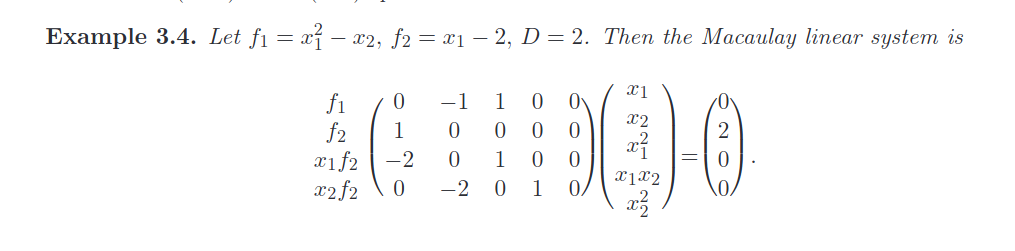
\includegraphics[width=14cm]{Macaulay.png}
  \caption{Example for a simple Macaulay Matrix.\label{abb_1}}
\end{figurehere}
\vspace{0.3cm}

\noindent
\textbf{Definition 3.2.5} \\
Let $A$ be a complex matrix, $A \in \mathbb{C}^{M,N}$, and its complex conjugate transpose $A^\intercal \in \mathbb{C}^{N,M}$. The singular values of $A, \, s_1 \geq s_2 \geq,...,\geq s_p \geq 0, \, p = min(M,N)$, are defined to be the positive square roots of the eigenvalues of $AA^\intercal$, if $\mathcal{M} \leq \mathcal{N}$, written

$$\sqrt{\lambda_i AA^\intercal}$$

\noindent
and those of $A^\intercal A$, if $\mathcal{M} \geq \mathcal{N}$. \\

\noindent
The \textbf{condition number} $\kappa(A) := \frac{s_{max}}{s_{min}}$ is the quotient of the maximal and minimal singular values. \\

\noindent
\textbf{Definition 3.2.6} \\
Given $f: \mathbb{C}^M \Rightarrow \mathbb{C}^M$, we denote by $Eig(f,\lambda)$ the eigenspace of $f$ associated with the eigenvalue $\lambda$. \\

\noindent
The dimension-formula for linear maps $f: \mathbb{C}^N \Rightarrow \mathbb{C}^N$ says that $dim \, ker(f) + rank(f) = N$. So $Eig(f,0) = ker(f)$ (the kernel of $f$). Now, let $A = A_{F,D} \in \mathbb{C}^{\mathcal{M} \times \mathcal{N}}$ ($F,D$ are arbitrary) be one of the modified Macaulay matrices constructed by Chen-Gao as above. Then we consider the linear map $f: \mathbb{C}^M \Rightarrow \mathbb{C}^M$, induced by the matrix $AA^\intercal = f$, and our result is: \\

\noindent
\textbf{Theorem 3.2.7} \\
$\kappa(A)=\infty$. \\

\noindent
\textbf{Proof of Theorem 3.2.7} \\
First note that $A$ has at least one $0$-row and one $0$-column by remarks 3.3 and 3.4 (Actually, for this proof, the existence of a $0$-row OR a $0$-column is sufficient.) Then $AA^\intercal = f$ has at least one $0$-row, too, by matrix multiplication. Then $rank(f) \leq M-1$, and by the dimension-formula for linear maps, it follows that $dim \,ker(f) + rank(f) \leq dim \,ker(f) + M-1$, so $M \leq dim \,ker(f) + M-1$.\\
Assume that $dim \,ker(f) = 0$, then it also holds that $M \leq M-1$, which is a contradiction. Therefore we have $dim \,ker(f) \geq 1$ and  $dim \,Eig(f,0) \geq 1$, 
which in turn means, that $f$ has the eigenvalue $\lambda = 0$. So $A$ has the singular value $s = 0 = s_{min}$, the minimal singular value, and
$k(A) = \frac{s_{max}}{s_{min}} = \infty$. \\

\noindent
\textbf{Theorem 3.2.8} \\
$\kappa(A_{mca}(S$-Box$))=\infty$, the condition number of the whole polynomial system $F$ is infinite. \\

\noindent
\textbf{Proof of Theorem 3.2.8} \\
In the paper \cite{QAA}, algorithm 4.2 has the following properties: The runtime complexity of the algorithm is  $\mathcal{O}(n^{2.5}(n + T_F)\kappa^2 \log(\frac{1}{\epsilon})$, where $\kappa$ is the maximal condition number for all matrices $A_{\mathcal{F}_2,D}$ in Step $4$, called the CONDITION NUMBER $\kappa(F) = \kappa)$ for the polynomial system $F$. By their Lemma 4.5, there are at most $n$ iterations in the loop, where the matrices $A_{\mathcal{F}_2,D}$ are used. Since all their condition numbers are infinite, the condition number of the polynomial system is infinite as well, and so is the runtime complexity of the Chen-Gao-Algorithm (Theorem 4.3). \\

\noindent
\textbf{Parameters of the S-Box in \textsc{AES}:} \\
We shall show that in this case, $A_{\mathcal{F},D}$ is of dimension $( \geq 10^{500} \times \geq 10^{500})$, and that the number of entries $\neq 0$ is only $\leq 10^6$ (total sparseness of $A_{mca}(S$-Box)), thus proving that there exist at least one $0$-row and at least one $0$-column in the Macaulay matrix $A_{mca}(S$-Box).\\

\noindent
We use table $2$ in \cite{QAA}, page $26$ to calculate the parameters of $A_{mca}(S$-Box). The $S$-Box is a \textit{Boolean multivariate quadratic equation system (BMQ)} with $d = 2,\,\, \overline{d} := min \{d \geq 0,\, d + 1 = 2^\delta\}$ for some  $\delta \in \mathbb{N}$. So $\delta = 1, \, d + 1 = 2$, and therefore $\overline{d} = 1$. Furthermore $\overline{D}:= min \{D \geq 2, \, D + 1 = 2^\Delta\}$ for some $\Delta \in \mathbb{N}$. So $\Delta = 2, \, d + 1 = 2^2$, and therefore $\overline{D} = 3$. \\

\noindent
The number of equations $r$ of the \textit{BMQ} is $4400$, and the number of variables $n \geq 1792$. \\
So we have for $\mathcal{M}$, the number of rows in $A_{mca}(S$-Box): $\mathcal{M} \geq 4400 \cdot 2^{1792} > 10^{500}$.\\
And for $\mathcal{N}$, the number of columns in $A_{mca}(S$-Box), we have: $\mathcal{N} \geq 4^{1792} > 10^{500}$. \\

\noindent
The number of entries $\neq 0 = 1$ equals the $\mathcal{T}$-sparseness in table $2$ on page $26$ of \cite{QAA}. This is at most $696\,384 < 10^6$ for \textsc{AES}-$256$. On the other side, even if we have $500\,000$ ones and zeros in separate rows and columns, there must at least exist one $0$-row and one $0$-column in $A_{mca}(S$-Box).\\ 


\section{Intermediary Conclusion and Next Steps}

\noindent
The conclusion of \cite{QAA} is, that systems which can be solved by Boolean equation solving, are only secure under quantum algebraic attack, if the condition number $\kappa$ is large. The complexity of $2^{78.53}c\kappa^2$ for \text{AES}-$256$ is not much higher than the complexity of $2^{73.30}c\kappa^2$ for \text{AES}-$128$ due to the same block size of $128$ bit.\\
The condition number $\kappa = \infty$ of $A_{mca}(S$-Box) in \textsc{AES} does not depend on the key size. It implies that the complexity of the quantum algebraic attack on \textsc{AES} equals infinity as well, if only the classical notion of the condition number of a matrix is considered. \\

\noindent
The consideration of the modified notion of a condition number, which allows ignoring zero singular values of a Boolean Equation System, requires the explicit generation of the involved reduced Macaulay matrix and the computation of its condition number. These investigations are currently ongoing in our independent research project. \\

\noindent
Besides \textsc{AES} and \textsc{Keccak}, stream ciphers such as \textsc{Trivium} and the multivariate public key cryptosystem \textsc{MPKC} are affected by the attack. The condition numbers of those Macaulay systems remain to be investigated.\\

\noindent
\textbf{Remark 4.1} \\
This paper is based on purely mathematical theorems, under the consideration of the classical notion of a condition number $\kappa$ of a matrix, and their corresponding mathematical proofs. By no means can we make a definite statement or prediction about: \\

\begin{itemize} [noitemsep, nolistsep]
  \item[1)] The modified notion of condition number of a matrix with zero eigenvalues, where the inversion takes only place on the orthogonal complement of the kernel \cite{SCH}. The modified condition number for \textsc{AES} remains to be investigated.
  \vspace{0.1cm}
  \item[2)] The potential physical outcome of an actual attack on \textsc{AES} with a quantum computer in the future under unforeseeable evolvements in mathematics or physics.\\
  \vspace{0.1cm}
\end{itemize}
\vspace{0.5cm}


\section{Context}

\subsection{Realization of Quantum Computing}

\noindent
With the advent of $49$ qubit processors quantum supremacy, the ability of quantum computing devices to solve problems that classical computers practically cannot solve,  lies within reach. IBM's $14$th quantum computer is its most powerful so far, a model with $53$ of the qubits that form the fundamental data-processing element at the heart of the system \cite{MSN}. Google participates in the race with their $72$-qubit quantum processor Bristlecone \cite{googleai}. \\

\noindent
The German Federal Office for Information Security (BSI) published a paper about the state of developments in quantum computing \cite{BSI}. They outline that the realization of potent quantum computers faces great challenges such as the scaling of needed qubits by error correcting codes and enormous hardware costs. \\
On the other hand, successful discoveries through research for \textit{topological quantum computation} \cite{TQB} might create a verbatim "quantum leap" in quantum computation evolvement, because they won't depend on error correcting mechanisms. Furthermore, adiabatic quantum computers, which work with \textit{quantum annealing mechanisms}, are already very successfully used for optimization problems.\\

\subsection{Hybrid Cryptosystems}

\noindent
With the availability of potent enough quantum computers, all private keys of asymmetric cryptosystems will be computable within reasonable time from the corresponding public keys. With the knowledge of those private keys, all encrypted data, which was collected and assigned to the relevant key exchanges, will no longer remain secret. \\

\noindent
Hybrid encryption systems combine the advantages of both cryptography classes, symmetric and asymmetric crypto systems. Asymmetric protocols allow securely sharing a key via digital connections, and symmetric protocols are about $10^5 \times$ faster than asymmetric ones. The secret session key \textit{SK}, whose validity is limited in time, is shared via asymmetric cryptography, and the message itself is symmetrically encrypted with the securely shared session key \textit{SK}. Hybrid cryptosystems are used in all major crypto protocols: TLS, SSH and PGP. They\\

\noindent
No asymmetric encryption within hybrid encryption systems can outbalance weaknesses of the symmetric part. ISO currently makes it possible to standardize new symmetric cryptography algorithms and to amend existing ones. Therefore, we strive to establish \textsc{eAES} as an ISO-Standard. Its predecessor \textsc{AES} has been standardized by both organizations. \\

\begin{figurehere}
  \centering
  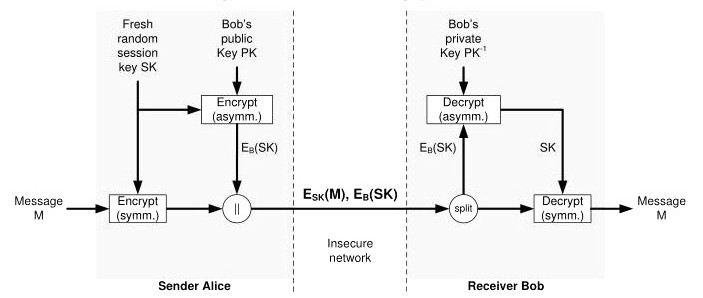
\includegraphics[width=12cm]{hybrid-encryption.jpg}
  \caption{Hybrid encryption.\label{abb_2}}
\end{figurehere}

\vspace{0.3cm} 





%%%%%%%%%%%%%%%%%%%%%%%%%%%%%%%%%%%%%%%%%%%%%%%%%%%%%%%%%%%%%%%%%%%%%%%%%%%%%%%%
% Literature
%%%%%%%%%%%%%%%%%%%%%%%%%%%%%%%%%%%%%%%%%%%%%%%%%%%%%%%%%%%%%%%%%%%%%%%%%%%%%%%%

\begin{thebibliography}{1}
\itemsep=0cm plus 0pt minus 0pt

\bibitem{QAA}
Y.~-A.~Chen, X.~-S.~Gao,
  \newblock Quantum Algorithms for Boolean Equation Solving and Quantum Algebraic Attack on Cryptosystems,
  \newblock {\em https://arxiv.org/pdf/1712.06239v3.pdf}, 2018.

\bibitem{AES}
Federal Information Processing Standards Publication 197, NIST,
  \newblock Announcing the ADVANCED ENCRYPTION STANDARD (AES),
  \newblock {\em https://csrc.nist.gov/csrc/media/publications/fips/\-197/final/documents/fips-197.pdf}, 2000.

\bibitem{GRV}
L.~K.~Grover,
  \newblock A fast quantum mechanical algorithm for database search, 
  \newblock { \em Gary L. Miller, editor, Proceedings of the
Twenty-Eighth Annual ACM Symposium on the Theory of Computing (STOC 1996), pages 212–219} ACM, 1996.

\bibitem{GRO}
M.~ Grassl, B.~ Langenberg, M.~ Roetteler, R.~ Steinwandt,
  \newblock Applying Grover’s algorithm to AES: quantum resource estimates,
  \newblock {\em https://arxiv.org/abs/1712.06239}, 2018.

\bibitem{KUN}
S.~Kovac and J.~Underhill,
  \newblock Towards post-quantum symmetric cryptography,
  \newblock {\em https://eprint.iacr.org/2019/553}.

\bibitem{QSH}
M.~Amy, O.~Di Matteo, V.~Gheorghiu, M.~Mosca, A.~Parent, J.~Schanck,
  \newblock Estimating the cost of generic quantum pre-image attacks on SHA-2 and SHA-3s, 
  \newblock { \em https://eprint.iacr.org/2016/992.pdf} QCrypt, 2016.

\bibitem{HHL}
A.W. Harrow, A.Hassidim, S.Lloyd, 
  \newblock Quantum algorithm for linear systems equations, 
  \newblock  { \em Physical Review Letters, 103(15)}: 150502, 2009. 

\bibitem{MCA}
F.S.M~acaulay, 
  \newblock Some formulas in elimination, 
  \newblock { \em Proc. Of the London Mathematical Society}, 35(1), 3-38, 1902. 

\bibitem{BDM}
K.~Batselier, P.~Dreesen, B.~De Moor, 
  \newblock On the null spaces of the Macaulay matrix, 
  \newblock { \em https://www.eee.hku.hk/~kimb/pdfs/MacaulayMatrix.pdf}.  


\bibitem{MSN}
  S.~Shankland,
  \newblock MSN News,
  \newblock { \em https://www.msn.com/en-us/news/technology/ibms-new-53-qubit-quantum-computer-is-its-biggest-yet/ar-AAHtPaW}, September 2019.

\bibitem{SCH}
  P.~Schleich,
  \newblock How to solve a linear system of equations using a quantum computer,
  \newblock { \em http://www.mathcces.rwth-aachen.de/\_media/3teaching/00projects/schleich.pdf}, July 2019.

\bibitem{googleai}
  J.~Kelly,
  \newblock Google AI Blog,
  \newblock {https://ai.googleblog.com/2018/03/a-preview-of-bristlecone-googles-new.html}, March 2018.

\bibitem{BSI}
BSI, Federal Office for Information Security Germany,
  \newblock Entwicklungsstand Quantencomputer
  \newblock { \em https://www.bsi.bund.de/SharedDocs/Downloads/DE/BSI/Publikationen/Studien/Quantencomputer/P283\_QC \\
  \_Studie.pdf, May 2018}

\bibitem{TQB}
  S.~Ran, C.~Eckberg, Q.-P.~Ding, Y.~Furukawa, T.~Metz, S.R.~Saha, I-L.~Liu, M.~Zic, H.~Kim, J.~Paglione and N.P.~Butch,
  \newblock NIST events on paper of above authors,
  \newblock { \em https://www.nist.gov/news-events/news/2019/08/newfound-superconductor-material-could-be-silicon-quantum-computers}.

\bibitem{CEX}
J.~Underhill,
  \newblock The CEX Cryptographic library in C++,
  \newblock {\em https://github.com/Steppenwolfe65/CEX}.

\bibitem{BUK}
X.~Bogomolec, J.~G.~Underhill, S.~A.~Kovac,
  \newblock Towards Post-Quantum secure symmetric Cryptography: 
A mathematical Perspective,  
  \newblock { \em Cryptology ePrint Archive: Report 2019/1208.}, 2019.


  
\end{thebibliography}

%%%%%%%%%%%%%%%%%%%%%%%%%%%%%%%%%%%%%%%%%%%%%%%%%%%%%%%%%%%%%%%%%%%%%%%%%%%%%%%%


%%% IF ENGLISH:
\end{otherlanguage}
%%%

\end{document}
